\documentclass{assignment}

% \textwidth=6.5in
% \hoffset-.75in
% \textheight=9in
% \voffset-.5in
\begin{document}

\title{5370 Midterm}
\author{Ritchie Cai}
\maketitle

Instructions.
\begin{itemize}
        \item The exam is due before class on October 15, 2015.
        \item Your solution is to be written in \LaTeX. The \LaTeX
        file and the corresponding pdf file is to be emailed to \verb"Robert_Marks@Baylor.edu" by the deadline.
        \item Show your work. Clarity of presentation counts.
        \item No human resource will be consulted in the execution of the exam.
        \item Problem~\ref{NewToyYoda} is really difficult. A successful solution might result in a publication. Be a Huffman!
\end{itemize}

\bigskip

% \documentclass{assignment}
\begin{document}

\title{5370 Midterm}

\textbf{1.} A random variable $X$ has the same probability of one third at the points $x=-1,0,1.$  Its entropy is thus $H_X = \log_2 3.$ Let $g(\cdot) $ denote a continuous function and define the random variable $Y=g(X)$.
\begin{enumerate} \item  Find a continuous function, $g(\cdot )$, that reduces the entropy of $Y$ to zero.
\item  Find another continuous function, $g(\cdot )$, that reduces the entropy of $Y$ below the entropy of $X$, but not to zero.
\item  Find a third function , $g(\cdot )$, that generates an entropy of $Y$ equal to the entropy of $X$.
\end{enumerate}
For all three answers, please sketch the nonlinearity and label your axes.


\end{document}
% \documentclass{assignment}
\begin{document}

\title{5370 Midterm}


\textbf{2.} Random variable are defined by the conditional probabilities
\begin{itemize}
\item  $\Pr[Y=1 | X=0] =q$
\item  $\Pr[Y=0 | X=1]=p$
\end{itemize}
where both $p$ and $q$ are fixed probabilities.
Assume $\Pr [X=0] =\pi $ where $\pi$ is some probability.
\begin{enumerate}
\item Calculate the mutual information between $X$ and $Y$.\\
  \textbf{Solutions:}\\
  Let
  \begin{align*}
    X_0 & = \{X=0\} \\
    X_1 & = \{X=1\} \\
    Y_0 & = \{Y=0\} \\
    Y_1 & = \{Y=1\}
  \end{align*}
  \begin{align*}
    \Pr[Y_1 | X_0] & = \df{\Pr[Y_1, X_0]}{\Pr[X_0]} = q \\
    \Pr[Y_1, X_0] & = \Pr[X_0]\; q = \pi q \\
    \Pr[X_0 | Y_1] & = \df{\Pr[Y_1, X_0]}{\Pr[Y_1]} = \df{\pi q}{\Pr[Y_1]}\\
    \Pr[Y_1] & = \Pr[Y_1 | X_0] + \Pr[Y_1 | X_1] = q + \Pr[Y_1 | X_1]\\
    \Pr[X_0 | Y_1] & = \df{\pi q}{q + \Pr[Y_1|X_1]} \\
    \\
    \Pr[Y_0 | X_1] & = \df{\Pr[Y_0, X_1]}{\Pr[X_1]} = p \\
    \Pr[Y_0, X_1] & = (1-\pi) p \\
    \Pr[X_1 | Y_0] & = \df{\Pr[X_1, Y_0]}{\Pr[Y_0]} = \df{(1-\pi)p}{\Pr[Y_0]} \\
    \Pr[Y = 0] & = \Pr[Y_0 | X_0] + \Pr[Y_0 | X_1] = \Pr[Y_0 | X_0] + p\\
    \Pr[X_1|Y_0] & = \df{(1-\pi) p }{\Pr[Y_0 | X_0] + p}
  \end{align*}
  \begin{align*}
    I(X;Y) & = \sum_{x,y}p(x, y) \log \df{p(x, y)}{p(x)p(y)} \\
           & = \Pr[X_0, Y_0] \log \df{\Pr[X_0, Y_0]}{\Pr[X_0]\Pr[Y_0]}
             + \Pr[X_0, Y_1] \log \df{\Pr[X_0, Y_1]}{\Pr[X_0]\Pr[Y_1]} +\\
           & \quad \Pr[X_1, Y_0] \log \df{\Pr[X_1, Y_0]}{\Pr[X_1]\Pr[Y_0]}
             + \Pr[X_1, Y_1] \log \df{\Pr[X_1, Y_1]}{\Pr[X_1]\Pr[Y_1]} \\
           % & = \Pr[X_0, Y_0] \log \df{\Pr[X_0, Y_0]}{\Pr[X_0]\Pr[Y_0]}
           %   + \pi q \log \df{q}{\Pr[Y_1]} + \\
           % & \quad (1-\pi)p \log \df{ p }{\Pr[Y_0]}
           %   + \Pr[X_1, Y_1] \log \df{\Pr[X_1, Y_1]}{\Pr[X_1]\Pr[Y_1]} \\
           % & = \Pr[X_0, Y_0] \log \df{\Pr[Y_0 | X_0]}{\Pr[Y_0]}
           %   + \pi q \log \df{q}{\Pr[Y_1]} + \\
           % & \quad (1-\pi)p \log \df{ p }{\Pr[Y_0]}
           %   + \Pr[X_1, Y_1] \log \df{\Pr[Y_1 | X_1]}{\Pr[Y_1]} \\
           & = \Pr[X_0, Y_0] \log \df{\Pr[Y_0 | X_0]}{\Pr[Y_0]}
             + \Pr[X_0, Y_1] \log \df{\Pr[Y_1 | X_0]}{\Pr[Y_1]} +\\
           & \quad \Pr[X_1, Y_0] \log \df{\Pr[Y_0 | X_1]}{\Pr[Y_0]}
             + \Pr[X_1, Y_1] \log \df{\Pr[Y_1 | X_1]}{\Pr[Y_1]} \\
           & = \Pr[Y_0, X_0]\log \Pr[Y_0 | X_0] - \Pr[Y_0, X_0] \log \Pr[Y_0] + \\
           & \quad \Pr[Y_1, X_0] \log \Pr[Y_1 | X_0] - \Pr[Y_1, X_0] \log \Pr[Y_1] + \\
           & \quad \Pr[Y_0, X_1] \log \Pr[Y_0 | X_1] - \Pr[Y_0, X_1] \log \Pr[Y_0] + \\
           & \quad \Pr[Y_1, X_1] \log \Pr[Y_1 | X_1] - \Pr[Y_1, X_1] \log \Pr[Y_1] \\
    % mod
           & = \Pr[Y_0, X_0]\log \Pr[Y_0 | X_0] - \Pr[Y_0, X_0] \log \Pr[Y_0] + \\
           & \quad \pi q \log q - \Pr[Y_1, X_0] \log \Pr[Y_1] + \\
           & \quad (1-\pi) p \log p - \Pr[Y_0, X_1] \log \Pr[Y_0] + \\
           & \quad \Pr[Y_1, X_1] \log \Pr[Y_1 | X_1] - \Pr[Y_1, X_1] \log \Pr[Y_1]
    \shortintertext{Still need:}
    \Pr[X_0, Y_0]           & \qquad \Pr[X_1, Y_1]\\
    \Pr[Y_0|X_0], \Pr[Y_0]  & \qquad \Pr[Y_1 | X_1], \Pr[Y_1]\\
    \Pr[X_0|Y_0]            & \qquad \Pr[X_1 | Y_1]
  \end{align*}

  \begin{align*}
    I(X ; Y) & = H(X) - H(X | Y) \\
           & = - \pi \log \pi - (1 - \pi) \log (1 - \pi)  - H(X | Y) \\
    H(X | Y) & = - \sum_{x, y} p(x, y) \log p(x | y) \\
             & = - \Pr[X_0, Y_0]\log \Pr[X_0 | Y_0] - \Pr[X_0, Y_1]\log \Pr[X_0 | Y_1] \\
             & \quad - \Pr[X_1, Y_0]\log \Pr[X_1 | Y_0] - \Pr[X_1, Y_1]\log \Pr[X_1 | Y_1] \\
             & = - \Pr[X_0, Y_0]\log \Pr[X_0 | Y_0] -  \pi q \log \df{\pi q}{\Pr[Y_1]} \\
             & \quad  - (1 - \pi) p \log \df{(1-\pi) p}{\Pr[Y_0]} - \Pr[X_1, Y_1]\log \Pr[X_1 | Y_1] \\
             & = - \Pr[X_0, Y_0]\log (\Pr[Y_0] - p) -  \pi q \log \df{\pi q}{\Pr[Y_1]} \\
             & \quad  - (1 - \pi) p \log \df{(1-\pi) p}{\Pr[Y_0]} - \Pr[X_1, Y_1]\log (\Pr[Y_1] - q)
  \end{align*}
\item What value of $\pi$ maximizes the mutual information?
\end{enumerate}

\end{document}


% \documentclass{assignment}
\title{5370 Midterm}

\begin{document}

\textbf{3.}
\label{SquishyBear}
The average word in English is $\lambda =5.1$ letters.
\begin{enumerate}
\item  If letters are drawn randomly from an $N=27$ character alphabet (A through Z and a space),\footnote{
    We are not considering punctuation, capitalization or numbers.
  }
  then when is a thick novel with $W$ words typical? Explain your reasoning. \\

  \textbf{Solution:} \\
  When
  \begin{align}
    p\left(X^{\ceil{W*(5.1 + 1)}}\right) & \approx 2^{-W*(5.1 + 1)*(5.1 + 1)} \label{problem3_1}
  \end{align}
  Because when n is very large, $E\left[\df{1}{n}l(X^n)\right] \approx H(X)$, which means $H(X) \approx \lambda$. The number of alphabets
  here, including space, should be about $\ceil{W * (\lambda + 1)}$, where ``+1'' is due the space character. Since
  we are adding space at the end of each words, the entropy for words with space should be $\lambda + 1$. So we have
  (\ref{problem3_1}), satisfying which makes the sequence at least weakly typical.

\item Here is a web page of 40,000 sampled words
  \begin{center}
    \verb"http://www.math.cornell.edu/~mec/2003-2004/cryptography/subs/frequencies.html"
  \end{center}
  \begin{enumerate}
  \item Complete the {\bf Count} column in table by including the {\em space}. Call the resulting empirical
    distribution $q(x)$ where $x=0,1,2,\cdots$ corresponds to (space, e, t, a, o, $\cdots$). \\
    \textbf{Solution:} \\
    Since sampled words are 40000, there should be the same amount of spaces, one space per word.

    \begin{tabular}[h]{l|l|r|r}
      Index & Letters & Count & Probability\\
      \hline
      0     & Space   & 40000 & 0.1799\\
      1     & E       & 21912 & 0.09857\\
      2     & T       & 16587 & 0.07461\\
      3     & A       & 14810 & 0.06662\\
      4     & O       & 14003 & 0.06300\\
      5     & I       & 13318 & 0.05991\\
      6     & N       & 12666 & 0.05698\\
      7     & S       & 11450 & 0.05151\\
      8     & R       & 10977 & 0.04938\\
      9     & H       & 10795 & 0.04856\\
      10    & D       & 7874  & 0.03542\\
      11    & L       & 7253  & 0.03263\\
      12    & U       & 5246  & 0.02360\\
      13    & C       & 4943  & 0.02224\\
      14    & M       & 4761  & 0.02142\\
      15    & F       & 4200  & 0.01889\\
      16    & Y       & 3853  & 0.01733\\
      17    & W       & 3819  & 0.01718\\
      18    & G       & 3693  & 0.01661\\
      19    & P       & 3316  & 0.01492\\
      20    & B       & 2715  & 0.01221\\
      21    & V       & 2019  & 0.009082\\
      22    & K       & 1257  & 0.005654\\
      23    & X       & 315   & 0.001417\\
      24    & Q       & 205   & 0.0009222\\
      25    & J       & 188   & 0.0008457\\
      26    & Z       & 128   & 0.0005758
    \end{tabular} \\

    After experiment, I found that beta-binomial distribution with $n=26, \alpha=0.68, \beta=2.7$ fit the data the best
    as shown in fig~\ref{fig:beta-binomial-fit}. Exponential distribution also fits well, but not as well as
    beta-binomial distribution, also exponential distribution is continuous, and beta-binomial is discrete which also
    make beta-binomial distribution a better fit.
    \begin{figure}[!h]
      \centering
      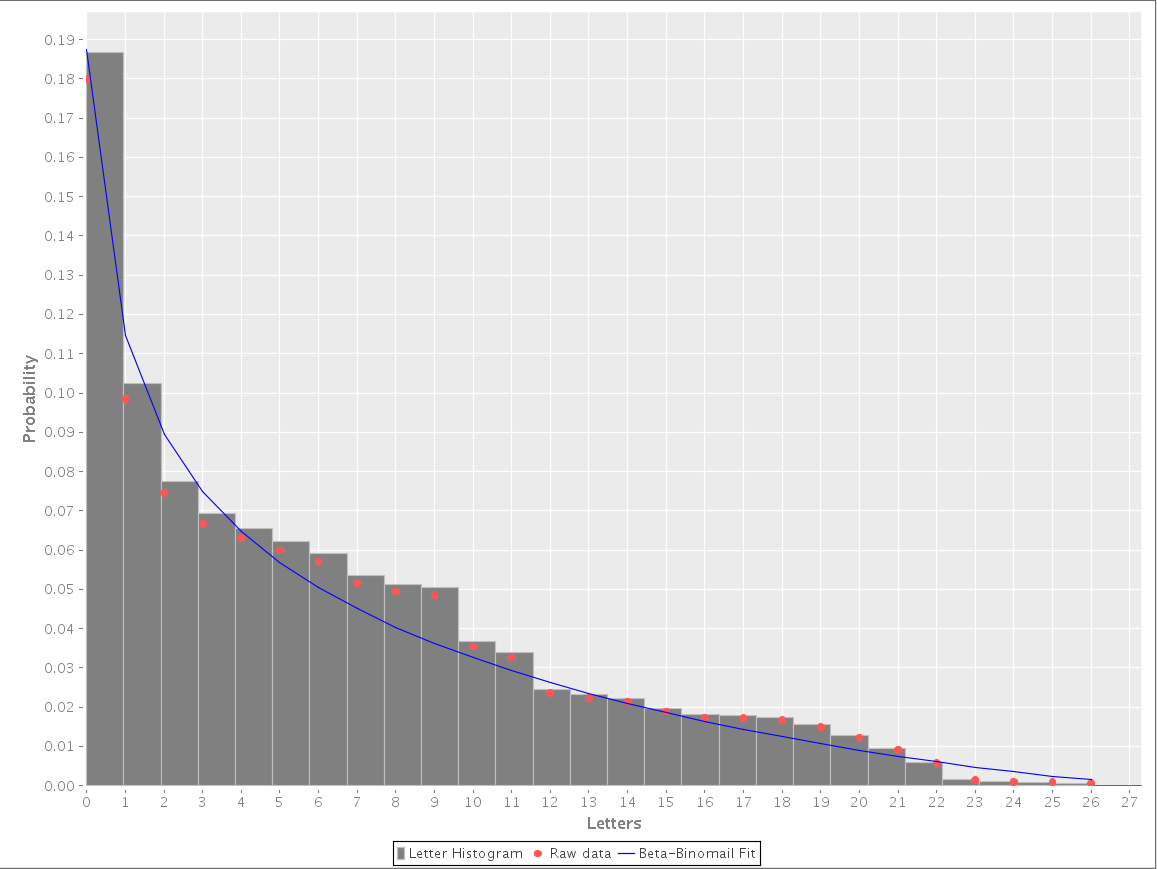
\includegraphics[width=5in]{pics/beta_binomial_fit.eps}
      \caption{Beta-binomial pmf fitting with $n=26, \alpha=0.68, \beta=2.7$}
      \label{fig:beta-binomial-fit}
    \end{figure}

  \item Find the value of $\alpha$ that minimizes the Kullback-Liebler distance between the distribution corresponding
    to this augmented table and
    \begin{align}
      p(x) = (1-\alpha) \alpha^x \label{eq:p3b_p(x)}
    \end{align}
    $$ $$ \\
    \textbf{Solutions:}\\
    Beta-binomial distribution pmf:
    \begin{align*}
      q(x|n, \alpha, \beta) & = \dbinom{n}{x} \df{B(x+\alpha, n-x+\beta)}{B(\alpha, \beta)} \\
      p(x) & = (1 - \alpha)\alpha^x
    \end{align*}
    Since we are assuming $q(x)$ as our true distribution and trying to make $p(x)$ as close to $q(x)$ as possible,
    by reducing KLIC, thus Kullback-Liebler distance should be expressed as:
    \begin{align*}
      D(q||p) & = \sum_x q(x)\log \df{q(x)}{p(x)} \\
      \shortintertext{Let}
      C_x & = \dbinom{n}{x} \\
      B_x & = B(x+\alpha, n-x+\beta) \\
      B   & = B(\alpha, \beta) \\
      \shortintertext{then we have:}
      D(q||p) & = \sum_x \dbinom{n}{x} \df{B(x+\alpha, n-x+\beta)}{B(\alpha, \beta)}
                \log \left(\df{\dbinom{n}{x} \df{B(x+\alpha, n-x+\beta)}{B(\alpha, \beta)}}{(1-\alpha)\alpha^x}\right) \\
              & = \df{1}{B}\sum_x C_xB_x\log\left( \df{\df{C_x B_x}{B}}{(1-\alpha)\alpha^x} \right) \\
              & = \df{1}{B}\sum_x \left[C_xB_x\log\left(\df{C_xB_x}{B}\right) - C_xB_x\log ((1-\alpha)\alpha^x)\right] \\
              & = \df{1}{B}\sum_x C_xB_x\log\left(\df{C_xB_x}{B}\right) - \df{1}{B}\sum_x C_xB_x\log ((1-\alpha)\alpha^x)
    \end{align*}
    As we can see, the function of $D(q||p)$ contains a inverted log function with respect to $\alpha$. Since log is a
    concave function, if there is a critical point exist, it must be a global minima. To find the critical point, we
    need to set $\df{d}{d\alpha} D(q||p) = 0$
    \begin{align*}
      \df{d}{d\alpha} D(q||p)
      & = \df{d}{d\alpha} \left(\df{1}{B}\sum_x C_xB_x\log\left(\df{C_xB_x}{B}\right)
                                - \df{1}{B}\sum_x C_xB_x\log ((1-\alpha)\alpha^x)\right) = 0 \\
      & = - \df{1}{B}\sum_x\df{C_xB_x(x\alpha^{(x-1)}-(x+1)\alpha^{x})}{(1-\alpha)\alpha^x} = 0\\
      & = - \df{1}{B}\sum_x\df{C_xB_x(x\alpha^{-1}-x-1)}{(1-\alpha)} = 0 \\
      & = \sum_x C_xB_x(x\alpha^{-1}-x-1) = 0 \\
      & = \sum_x C_xB_xx - \sum_x C_xB_x \alpha x - \sum_x C_xB_x\alpha = 0 \\
      \alpha & = \df{\sum_{x=0}^{26} C_xB_xx}{\sum_{x=0}^{26} C_xB_x (x + 1)}
               = \df{\sum_{x=0}^{26} \dbinom{n}{x}B(x+\alpha, n-x+\beta) x}
                    {\sum_{x=0}^{26} \dbinom{n}{x}B(x+\alpha, n-x+\beta) (x + 1)} \\
      \shortintertext{with $n=26, \alpha=0.68, \beta=2.7$}
      \alpha & \approx 0.8395
    \end{align*}

    % \begin{align*}
    %   q(x) & = \df{\lambda^x}{x!}e^{-\lambda} = \df{\lambda^x}{x! e^{\lambda}} \\
    %   p(x) & = (1-\alpha) \alpha^x
    % \end{align*}
    % \begin{align*}
    %   D(p||q) & = \sum_x p(x)\log \df{p(x)}{q(x)}\\
    %           & = \sum_{x=0}^{26} (1-\alpha) \alpha^x \log \df{x!e^{\lambda}(1-\alpha) \alpha^x}{\lambda^x} \\
    %           & = \sum_{x=0}^{26} \left[(1-\alpha) \alpha^x\log \df{x!e^{\lambda}}{\lambda^x}
    %             + (1-\alpha) \alpha^x\log (1-\alpha) \alpha^x\right]
    % \end{align*}
    % Since this is a function contains an odd degree of polynomial function, $\left.a^{x+1}\right|_{x=26}$, this function
    % has no global minimum or global maximum. So we have to use (\ref{eq:p3b_p(x)}) as our true distribution.

    % \begin{align*}
    %   D(p||q) & = \sum_x p(x)\log \df{p(x)}{q(x)}\\
    %        & = \sum_{x=0}^{26} (1-\alpha) \alpha^x \log \df{x!e^{\lambda}(1-\alpha) \alpha^x}{\lambda} \\
    %   \shortintertext{for $x=0$:}
    %   \df{d}{d\alpha}\left((1-\alpha) \log\df{e^{\lambda}(1 - \alpha)}{\lambda}\right)
    %           & = -\log\df{e^{\lambda}(1 - \alpha)}{\lambda}
    %             - \df{e^{\lambda}(1 - \alpha)}{\lambda} \df{\lambda}{e^{\lambda}(1 - \alpha)} \\
    %           & = -\log\df{e^{\lambda}(1 - \alpha)}{\lambda} - 1 \\
    %  \end{align*}
    %  \begin{align*}
    %   \shortintertext{for $x = 1, 2, \dots, 26$, let:}
    %   T & = (1-\alpha) \alpha^x \log \df{x!e^{\lambda}(1-\alpha) \alpha^x}{\lambda} \\
    %        & = \alpha^x\log \df{x!e^{\lambda}(1-\alpha) \alpha^x}{\lambda} -
    %          \alpha^{x+1}\log \df{x!e^{\lambda}(1-\alpha) \alpha^x}{\lambda} \\
    %   \df{d}{d\alpha} T
    %        & = xa^{x-1}\log \df{x!e^{\lambda}(1-\alpha) \alpha^x}{\lambda}
    %          + a^x \left( \df{x!e^{\lambda}}{\lambda} \right)
    %          \df{(-a^x + x(1 - \alpha)\alpha^{x-1})\lambda}{x!e^{\lambda}(1-\alpha) \alpha^x} \\
    %        & \quad - (x+1)\alpha^x\log \df{x!e^{\lambda}(1-\alpha) \alpha^x}{\lambda}
    %          - a^{x+1} \left( \df{x!e^{\lambda}}{\lambda} \right)
    %          \df{(-a^x + x(1 - \alpha)\alpha^{x-1})\lambda}{x!e^{\lambda}(1-\alpha) \alpha^x} \\
    %        & = xa^{x-1}\log \df{x!e^{\lambda}(1-\alpha) \alpha^x}{\lambda}
    %          + \df{-a^x + x \alpha^{x-1} - x\alpha^x}{(1-\alpha)} \\
    %        & \quad - (x+1)\alpha^x\log \df{x!e^{\lambda}(1-\alpha) \alpha^x}{\lambda}
    %          - \df{-a^{x+1} + x(1 - \alpha)\alpha^{x}}{1-\alpha} \\
    %        & = (x a^{x-1} - (x+1) \alpha^x)\log \df{x!e^{\lambda}(1-\alpha) \alpha^x}{\lambda}
    %          + \df{-a^x + x \alpha^{x-1} - x\alpha^x + a^{x+1} - x(1 - \alpha)\alpha^{x}}{1-\alpha}
    % \end{align*}

    % \begin{align*}
    %   D(q || p) & = \sum_x q(x) \log \df{q(x)}{p(x)} \numberthis \label{eq:p3b_KLD}\\
    %             & = \sum_x \df{\lambda}{x!e^{\lambda}}\log \df{\lambda}{x!e^{\lambda} (1-\alpha)\alpha^x} \\
    %             & = \sum_x \df{\lambda}{x!e^{\lambda}}(\log \lambda - \log (x! e^{\lambda}(1 - \alpha) \alpha^x)) \\
    %             & = \df{27\lambda}{x!e^{\lambda}} - \sum_{x=0}^{26} \log (x! e^{\lambda}(1 - \alpha) \alpha^x)
    % \end{align*}
    % Since log is a concave function and this particular one is a inverted log function, if there is a point where
    % derivative is 0, it must be a global minimum.
    % \begin{align*}
    %   \df{d}{d\alpha} D(q || p) & = - \sum_{x=0}^{26} \df{x x!e^{\lambda}a^{x-1} - (x+1)!e^{\lambda}a^x}
    %                                                     {x!e^{\lambda}(1-\alpha)\alpha^x} \\
    %                             & = - \sum_{x=0}^{26} \df{x a^{-1} - (x+1)}{1-\alpha} \\
    %                             & = \df{\sum_{x=0}^{26}[x - \alpha(x + 1)]}{\alpha^2 - \alpha} = 0 \\
    %   \sum_{x=0}^{26}[x - \alpha(x + 1)] & = 0 \\
    %   \alpha\sum_{x=0}^{26}(x + 1) & = \sum_{x=0}^{26} x \\
    %   \alpha & = \df{\sum_{x=0}^{26} x}{\sum_{x=0}^{26}(x + 1)} = \df{13}{14}
    % \end{align*}
    % So, when $\alpha = \frac{13}{14}$, (\ref{eq:p3b_KLD}) has the smallest value.

  \item Compare this to the $\alpha$ that minimizes
    $$ \sum_{x=0}^\infty \left| p(x) -  q(x) \right|^2 $$ \\
    \textbf{Solution:} \\
    Since we only have $0-26$, i.e., 26 alphabets with one space character, the summation would only go up to 26, reset
    of terms would be all 0
    \begin{align*}
      \sum_{x=0}^{26} \left| p(x) -  q(x) \right|^2
      & = \sum_{x=0}^{26} \left| (1- \alpha) \alpha^x - \df{C_xB_x}{B}\right|^2 \\
      & = \sum_{x=0}^{26} \left| a^x - a^{x+1} - \df{C_xB_x}{B}\right|^2 \\
      & = \sum_{x=0}^{26} \left(  a^{2x} - a^{2x+1} - \df{C_xB_x}{B}a^x \right. \\
      & \quad \quad \quad \quad - a^{2x+1} + a^{2x+2} + \df{C_xB_x}{B}a^{x+1} \\
      & \quad \quad \quad \quad \left. - \df{C_xB_x}{B}a^{x} + \df{C_xB_x}{B}a^{x+1} + \left(\df{C_xB_x}{B}\right)^2
        \right) \\
      & = \sum_{x=0}^{26} \left(a^{2x+2} - 2a^{2x+1} + a^{2x} + \df{2C_xB_x}{B}a^{x+1} - \df{2C_xB_x}{B}a^{x} +
        \left(\df{C_xB_x}{B} \right)^2 \right) \numberthis \label{eq:prob3c:f}\\
      & = \sum_{x=0}^{26} \left(a^{2x+2} - 2a^{2x+1} + a^{2x}\right)
        + \sum_{x=0}^{26} \left( \df{2C_xB_x}{B}a^{x+1} - \df{2C_xB_x}{B}a^{x} +
        \left(\df{C_xB_x}{B} \right)^2 \right) \numberthis \label{eq:prob3c:f3}\\
      % & = \sum_{x=0}^{26} \left((a - 1)^2 a^{2x}  + \df{2C_xB_x}{B} a^{x+1} - \df{2C_xB_x}{B} a^x
      %   + \left(\df{C_xB_x}{B}\right)^2\right) \\
      % & = \sum_{x=0}^{26} a^{2x}(a - 1)^2
      %   + \sum_{x=0}^{26} \left(  \df{2C_xB_x}{B} a^{x+1} - \df{2C_xB_x}{B} a^x + \left(\df{C_xB_x}{B}\right)^2\right) \\
      % & = \sum_{x=0}^{26} (a^{2x+2} - 2a^{2x+1} + a^{2x})
      %   + \sum_{x=0}^{26} \left( 2C_xB_x a^{x+1} - 2C_xB_x a^x + \df{(C_xB_x)^2}{B}\right)
      %   \numberthis \label{eq:prob3c:f2} \\
    \end{align*}
    Since this is a polynomial with even degree and positive leading coefficient, $a^{2\times 26 + 2} = a^{54}$, the
    opening of the polynomial should be upward and it should have at least one global minimum.

    With first and second derivative of (\ref{eq:prob3c:f}):
    \begin{align*}
      \df{d}{da}\left(\sum_{x=0}^{26} \left| p(x) -  q(x) \right|^2\right)
      & = \sum_{x=1}^{26} \left( (2x+2)a^{2x+1} - (4x+2)a^{2x} + 2xa^{2x-1}\right) \\
      & \quad + \sum_{x=1}^{26} \left( (x+1)\df{2C_xB_x}{B} a^{x} - x\df{2C_xB_x}{B} a^{x-1}\right)
        + 2a -2 + \df{2C_0B_0}{B} \\
      \df{d^2}{da^2}\left(\sum_{x=0}^{26} \left| p(x) -  q(x) \right|^2\right)
      & = \sum_{x=2}^{26}  \left((2x+2)(2x+1)a^{2x} - (2x+2)2xa^{2x-1} + 2x(2x-1)a^{2x-2}\right) \\
      & \quad  + \sum_{x=2}^{26} \left( x(x+1)2\df{C_xB_x}{B} a^{x-1} - x(x-1)2\df{C_xB_x}{B} a^{x-2}\right) \\
      & \quad + 12a^2 - 12a + 2 + \df{4C_1B_1}{B} + 2
    \end{align*}
    we can numerically find the global minimum(s) with Newton's
    method\footnote{\url{https://en.wikipedia.org/wiki/Newton\%27s_method}} which gives me $\alpha \approx 0.83495$.
    Code used for newton's method is shown
    in listing (\ref{lst:newton}) and (\ref{lst:binomial})
    \SourceCode{clojure}{Functions for using newton's method}{lst:newton}{../../src/elc5370/optimization.clj}
    \SourceCode{clojure}{Functions for beta binomial distribution}{lst:binomial}{../../src/elc5370/binomial.clj}
    % \begin{align*}
    %   & = (a - 1)^2\sum_{x=0}^{26} 2xa^{2x-1} + \df{1}{B}\sum_{x=0}^{26} \left(2C_xB_x(x+1)a^{x} - 2C_xB_xxa^{x-1}\right)
    % \end{align*}

  \item What is the average word length in English based on $q(x)$? On $p(x)$? \\
    \textbf{Solution:} \\
     Ideally,
     \begin{align*}
       \text{average word length} & = \df{\text{total length (or non-space characters count)}}
                                         {\text{number of words (or spaces)}}
                                    = \df{\text{182303}}{\text{40000}}
                                    \approx 4.56
     \end{align*}
     However, average length based on a distribution $f(x)$, in general, should be
     \begin{align*}
       \text{average word length} & = \df{\sum_{x=1}^{26} f(x)}{f(x=0)}
     \end{align*}
     So, for $q(x)$, we have:
     \begin{align*}
       \text{average word length} & = \df{\sum_{x=1}^{26} q(x)}{q(0)} \approx \df{0.8066}{0.1935} \approx 4.17 \\
       \shortintertext{where}
       q(x) & = \dbinom{n}{x} \df{B(x+\alpha, n-x+\beta)}{B(\alpha, \beta)}
              \quad \text{with $n = 26, \alpha = 0.68, \beta = 2.7$}
     \end{align*}
     For $p(x)$, we have:
     \begin{align*}
       \text{average word length} & = \df{\sum_{x=1}^{26} p(x)}{p(0)} \approx \df{0.8306}{0.1605} \approx 5.18 \\
       \shortintertext{where}
       p(x) & = (1- \alpha)\alpha^x \quad \text{with $\alpha$ = 0.8395}
     \end{align*}
  \end{enumerate}
\end{enumerate}


\end{document}

\documentclass{assignment}
\title{5370 Midterm}
\author{Ritchie Cai}


\begin{document}


\textbf{4.} Problem 2.10b in the text:\\
\begin{align*}
  H(X) & = -\alpha\log\alpha - (1 - \alpha)\log (1- \alpha) + \alpha H(X_1) + (1 - \alpha) H(X_2)
\end{align*}
Maximize over $\alpha$ to show that $2^{H(X)}\leq 2^{H(X_1)} + 2^{H(X_2) }$ and interpret using the notion that $2^{H(X)}$ is the effective alphabet size.\\

\textbf{Solution:} \\
\begin{align*}
  \df{d}{d\alpha} H(X)
  & = \df{d}{d\alpha}\left[ -\alpha\log\alpha - (1 - \alpha)\log (1- \alpha) + \alpha H(X_1) + (1 - \alpha) H(X_2)\right]
    = 0 \\
  & = -\left(\log \alpha + \alpha \df{1}{\alpha}\right) - \left( - \log(1-\alpha) - (1-\alpha)\df{1}{1-\alpha}\right)
      + H(X_1) - H(X_2)\\
  & =  -\log\alpha - 1 + \log(1-\alpha) + 1 + H(X_1) - H(X_2) \\
  & =  \log(1-\alpha) - \log\alpha + H(X_1) - H(X_2) \\
  & = \log\left( \df{1 -\alpha}{\alpha} \right) + H(X_1) - H(X_2) = 0\\
  \Rightarrow \log\left( \df{1 -\alpha}{\alpha} \right) & = H(X_2) - H(X_1) \\
  \df{1 - \alpha}{\alpha} & = 2^{H(X_2) - H(X_1)} \\
  1 & = \alpha 2^{H(X_2) - H(X_1)} + \alpha\\
  1 & = \alpha \left( 2^{H(X_2) - H(X_1)} + 1 \right) \\
  \alpha & = \df{1}{2^{H(X_2) - H(X_1)} + 1} = \df{1}{K + 1} \\
  \shortintertext{where:}
  K & = 2^{H(X_2) - H(X_1)}
\end{align*}
So we have:
\begin{align*}
  1 - \alpha & = 1 - \df{1}{K + 1} = \df{K}{K + 1} \\
  H(X) & = - \df{1}{K + 1} \log\left( \df{1}{K + 1} \right) - \df{K}{K + 1}\log\left( \df{K}{K + 1} \right)
           + \df{1}{K + 1} H(X_1) + \df{K}{K + 1}H(X_2) \\
             & = \df{\log(K + 1) - K\log\left( \df{K}{K + 1} \right) + H(X_1) + K H(X_2)}{K + 1} \\
             & = \df{\log(K + 1) - K\log(K) + K\log(K+1) + H(X_1) + K H(X_2)}{K + 1} \\
             & = \df{H(X_1) +K H(X_2) - K\log(K)}{K+1} + \log(K+1) \\
  \shortintertext{let $a=H(X_1)$, $b=H(X_2)$}
  H(X) & = \df{a +2^{b - a} b - 2^{b - a}\log(2^{b - a})}{2^{b - a}+1} + \log(2^{b - a}+1)
             % & = \df{\log(K + 1) + K\log\left( \df{K + 1}{K} \right) + H(X_1) + K H(X_2)}{K + 1} \\
             % & = \df{\log(K + 1) + K\log\left( 1 + \df{1}{K} \right) + H(X_1) + KH(X_2)}{K + 1}
\end{align*}

% \begin{align*}
%   \shortintertext{Since:}
%   \log (a + b) & = \log(a * (1 + b/a)) \\
%   \shortintertext{We have:}
%   \log(K + 1) & = \log\left(K * \left(1 + \df{1}{K}\right)\right)\\
%                & = K + \log\left(1 + \df{1}{K}\right) \\
% \end{align*}
% So,
% \begin{align*}
%   H(X) & = \df{K + \log\left(1 + \df{1}{K}\right)
%          + K\log\left( 1 + \df{1}{K}
%          \right) + H(X_1) + KH(X_2)}{K + 1} \\
%        & = \df{K + \log\left(1 + \df{1}{K}\right)\left( 1 +  K\right)
%          + H(X_1) + KH(X_2)}{K + 1} \\
%        & = \df{K + H(X_1) + KH(X_2)}{K + 1}
%            + \log\left(\df{K + 1}{K}\right)
% \end{align*}
\end{document}

% \documentclass{assignment}
\begin{document}

\title{5370 Midterm}


\textbf{5.} \label{NewToyYoda}
Continuation from Problem~\ref{SquishyBear}.
The distribution of English word length, $k$, is a shifted Poisson random variable. At the end of each word, we will add
a space to separate words. There are no spaces allowed in the middle of a word. Under this assumption word length
follows the distribution
\begin{align}
  w(k)=\frac{e^{-\lambda}\lambda^{k-2} }{(k-2)!} ; k=2,3,4,\cdots \label{eqn:problem5:length}
\end{align}
$$ $$
Assuming there are about a million words in the English language.
\begin{enumerate}
\item What is the probability of generating a word in the English language randomly choosing letters
  \begin{itemize}
  \item assuming the letters are chosen uniformly.
  \item assuming the letters are chosen according to $p(x)$.\footnote{See Problem~\ref{SquishyBear}.}
  \end{itemize}
  \textbf{Solution:} \\
  \begin{align*}
    \text{Let} \quad & \begin{cases}
      K & = \text{probability of generating a sequence of non-space alphabets followed by a space
      character} \\
      E & = \text{probability of generating a valid English word} \\
      N & = \text{total number of English words}, 1000000
    \end{cases}
  \end{align*}
  Using conditional probability relation we can express $\Pr\{E\}$ as:
  $$\Pr\{E\}= \sum_k \Pr\{E \cap K\} = \sum_k \Pr\{E|K=k\}\Pr\{K=k\}$$
  where
  $$\Pr\{K=k\} = (1 - \Pr\{\text{space}\})^{k-1}\Pr\{\text{space}\}$$

  Since $w(k) * N \approx $ number of English words with length $k$, we can express $\Pr\{E|K=k\}$ as
  $$\Pr\{E|K=k\} \approx \df{w(k) * N}{26^{k-1}\times 1}$$

  However, when $k=2,3,4$, using (\ref{eqn:problem5:length}) gives us unexpected word counts:
  \begin{align*}
    w(2) & = \df{e^{-6.1}6.1^0}{0!} \approx 0.0060967 \\
    w(2) * 1000000 &  \approx 2242 > 26 \\
    w(3) & = \df{e^{-6.1}6.1^1}{1!} \approx 0.013681 \\
    w(3) * 1000000 & \approx 13681 > 26^2 \\
    w(4) & = \df{e^{-6.1}6.1^2}{2!} \approx 0.041729 \\
    w(4) * 1000000 & \approx 41728 > 26^3
  \end{align*}
  Note that I am using $\lambda = 6.1$ since we are adding an additional space at the end of each word.


  For this reason, in order to get a reasonable estimation, I will use some data I found online for $k=2,3,4$ terms. 

  According to Wikipedia,
  \begin{itemize}
  \item Number of 1 letter-words = 3\\
    source: \url{https://en.wiktionary.org/wiki/Category:English_one-letter_words}
  \item Number of 2 letter-words = 114\\
    source: \url{https://en.wiktionary.org/wiki/Category:English_two-letter_words}
  \item Number of 3 letter-words = 172\\
    source: \url{https://en.wiktionary.org/wiki/Category:English_three-letter_words}
  % \item Number of 4 letter not-words = 2745\\
  %   source: \url{http://www.appsapps.info/stuff/notwords4.txt}
  \end{itemize}

  Thus, my estimation for generating a word in English is:
  \begin{align*}
    \Pr\{E\} & = \sum_{k=2}^{N} \left(\df{w(k) * N}{26^{k-1}}
               (1 - \Pr\{\text{space}\})^{k-1}\Pr\{\text{space}\}\right) \\
    \Pr\{E\} & = \df{3}{26}(1 - \Pr\{\text{space}\})\Pr\{\text{space}\} + \\
             & \quad \df{114}{26^2}(1 - \Pr\{\text{space}\})^2\Pr\{\text{space}\} + \\
             & \quad \df{172}{26^3}(1 - \Pr\{\text{space}\})^3\Pr\{\text{space}\} + \\
             & \quad \sum_{k=5}^{N} \left(\df{w(k) * N}{26^{k-1}}
               (1 - \Pr\{\text{space}\})^{k-1}\Pr\{\text{space}\}\right)
  \end{align*}
  % For $\Pr\{E|K=k\}$, it's the probability of English word when given a sequence of non-space alphabets
  % followed by a space. So it can be computed with number of English words in a given length divided by
  % all the possible combination of non-space alphabets in that given length. Since we know the total
  % number of English words and the
  So,
  \begin{itemize}
    \item If letters are chosen uniformly,
      \begin{align*}
        \Pr\{\text{space}\}
        & = \df{1}{27} \\
        \Pr\{E\}
        & = \sum_{k=2}^{N} \left(\df{w(k) * N}{26^{k-1}}\left( \df{26}{27} \right)^{k-1}\df{1}{27}\right) \\
        & = \sum_{k=2}^{N} \left(\df{w(k) * N}{27^{k}} \right) \\
        & = \df{3}{27^2} + \df{114}{27^3} + \df{172}{27^4} +
          \sum_{k=5}^{N} \left(\df{w(k) * N}{27^{k}} \right) \\
        & \approx 0.01649 \numberthis \label{result:prob5:1}
      \end{align*}
    \item If letters are chosen according to $p(x)$,
      \begin{align*}
        \Pr\{\text{space}\}
        & = \df{40000}{222303} \approx 0.17993 \\
        \Pr\{E\} & = \df{3}{26} \df{182303}{222303} \df{40000}{222303} +
                   \df{114}{26^2} \left(\df{182303}{222303}\right)^2 \df{40000}{222303} +
                   \df{172}{26^3} \left(\df{182303}{222303}\right)^3 \df{40000}{222303} + \\
        & \quad \sum_{x=5}^{N} \left( \df{w(k) * N}{26^{k-1}}
          \left(\df{182303}{222303}\right)^{k-1} \df{40000}{222303} \right) \\
        & \approx 0.054269 \numberthis \label{result:prob5:2}
      \end{align*}

      \CodeSnippet{clojure}
      {Code used to compute the probability in (\ref{result:prob5:1}) and (\ref{result:prob5:2})}
      {lst:prob5:1}
      {../../src/elc5370/problem5.clj}{44}{68}

      % \begin{align*}
      %   P(W) & = \sum_{k=2}^{N} \left(\df{w(k) * N}{26^{k-1}} (1 - p(0))^{k-1}p(0)\right) \\
      %   P(W) & = \sum_{k=2}^{N} \left(\df{w(k) * N}{26^{k-1}}
      %          \left(1 - (1-\alpha)\alpha^0\right)^{k-1}(1-\alpha)\alpha^0\right) \\
      %        & = \sum_{k=2}^{N} \left(\df{w(k) * N}{26^{k-1}} \alpha^{k-1}(1-\alpha)\right) \\
      %        & = \sum_{k=2}^{N} \left(\df{w(k) * N}{26^{k-1}} p(k-1)\right)
      % \end{align*}
  \end{itemize}
  % % \url{http://www.languagemonitor.com/number-of-words/number-of-words-in-the-english-language-1008879/}
  % According to \url{http://www.languagemonitor.com}, $N \approx 1,025,109$

  % 4 letters non words \url{http://www.appsapps.info/stuff/notwords4.txt}

\item What is the probability of randomly generating $W$ words in a row under each distribution?\\
  \textbf{Solution:}\\
  \begin{itemize}
  \item If letters are chosen uniformly: $0.01649^W$
  \item If letters are chosen according to $p(x)$: $0.054269^W$
  \end{itemize}
\item How many times must we randomly sample before getting $W$ words in a row under each distribution?\\
  \textbf{Solution:}\\
  There is no guarantee that we can successfully choosing $W$ words randomly with any number 
  
\item If a word is $w_k$ characters long (including a space at the end), assume it requires $k \log_2 N$ bits to form. How many bits do we use, on average, to query to the point we have $W$ words in a row?
\end{enumerate}

\end{document}





\end{document}
